\section{اصول کار رادار \lr{FMCW}}\label{sec:fmcw-principles}


\subsection{سیگنال چیپ (\lr{Chirp}) و پهنای باند} % Subsection 2.1.1
\label{sec:chirp-bandwidth}

رادارهای \lr{FMCW (Frequency-Modulated Continuous Wave)} از نوع خاصی از امواج رادیویی استفاده می‌کنند که فرکانس آن‌ها به‌صورت خطی در بازه‌ای از زمان تغییر می‌کند. به این سیگنال‌ها، «چیپ» (\lr{Chirp}) گفته می‌شود. در یک چرخه از عملکرد رادار، سیگنال فرستاده‌شده از نوع خطی صعودی است که در آن فرکانس از یک مقدار آغازین \lr{$f_0$} تا مقدار \lr{$f_0 + B$} در مدت زمان \lr{$T$} افزایش می‌یابد.





\vspace{2cm}
\begin{center}
\begin{figure}[!h]
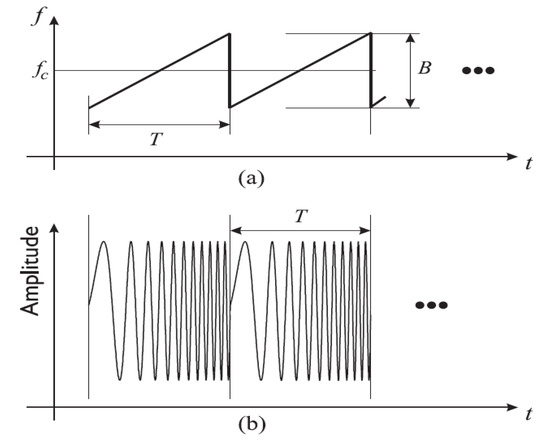
\includegraphics[height=10cm,width=12cm]{Images/chapter2/2-1.jpg}
\caption{(\lr{a}) تغییر فرکانس در طول زمان، (\lr{b}) سیگنال‌های \lr{chirp} لحظه‌ای.
\cite{kebe2020human}
}
\end{figure}
\end{center}
\vspace{2cm}

ویژگی کلیدی این نوع سیگنال در اندازه‌گیری فاصله، قابلیت نمایش موقعیت فاصله‌ای اهداف با استفاده از اختلاف فرکانسی بین سیگنال ارسال‌شده و سیگنال بازتابی است. هنگامی که سیگنال بازتابی از یک هدف با تأخیر زمانی دریافت می‌شود، اختلاف فرکانس بین سیگنال دریافتی و ارسال‌شده (که به آن \lr{beat frequency} گفته می‌شود) مستقیماً با فاصله هدف مرتبط است.


فرکانس \lr{beat} با رابطه زیر تعیین می‌شود:
\begin{equation}
f_b = \frac{2BR}{cT}
\label{eq:beat_frequency}
\end{equation}
\addequation{اختلاف فرکانس بین سیگنال دریافتی و ارسال‌شده}

که در آن:
\begin{itemize}
    \item \lr{$B$}: پهنای باند سیگنال چیپ
    \item \lr{$R$}: فاصله تا هدف
    \item \lr{$c$}: سرعت نور
    \item \lr{$T$}: مدت‌زمان سیگنال
\end{itemize}

 در کاربردهای زیستی مانند پایش ضربان قلب، حرکت‌های بسیار ظریف سطح قفسه سینه (در حد میلی‌متر یا کمتر) باعث ایجاد تغییرات فرکانسی بسیار کوچک در سیگنال برگشتی می‌شود، که با تحلیل دقیق این \lr{beat frequency} می‌توان علائم حیاتی نظیر ضربان قلب را استخراج کرد.
\cite{munoz2018doppler}

در مقاله \cite{neemat2019reconfigurable}، تمرکز بر افزایش قدرت تفکیک (\lr{resolution}) در محور فاصله است. طبق یافته‌های این مقاله، پهنای باند سیگنال چیپ مستقیماً بر توان تفکیک فاصله اثرگذار است.تفکیک فاصله‌ای \lr{$\Delta R$} به‌صورت زیر تعریف می‌شود:
\begin{equation}
\Delta R = \frac{c}{2B}
\label{eq:range_resolution}
\end{equation}
\addequation{رابطه‌ی تفکیک فاصله‌ای در رادار \lr{FMCW}}

بنابراین، افزایش پهنای باند باعث بهبود توانایی سیستم در تمایز اهداف نزدیک به هم می‌شود. در کاربردهای پزشکی مانند اندازه‌گیری ضربان قلب، که در آن سیگنال‌های بسیار ضعیف از حرکت‌های سطحی بدن ثبت می‌شود، این افزایش تفکیک می‌تواند به تفکیک بهتر نویز محیطی از سیگنال واقعی ضربان قلب منجر شود.
همچنین به معرفی پردازش دامنه داپلر قابل پیکربندی (\cite{neemat2019reconfigurable}) پرداخته است که با تغییر معماری فریم‌های چیپ، امکان جداسازی بهتر سیگنال‌های مربوط به تنفس و ضربان قلب فراهم می‌شود. این موضوع در شرایطی که حرکت‌های دیگر بدن وجود دارند (مانند تکان‌های سر یا دست)، اهمیت دوچندان پیدا می‌کند.
در جمع‌بندی این بخش، می‌توان گفت که استفاده از سیگنال‌های چیپ با پهنای باند بالا، نه‌تنها دقت فاصله‌سنجی را در رادارهای \lr{FMCW} افزایش می‌دهد، بلکه با بهره‌گیری از روش‌هایی مانند \lr{Range-Doppler} قابل پیکربندی، تفکیک و تحلیل دقیق‌تری از علائم حیاتی فراهم می‌آورد.

%=================================================================================================


\subsection{آشکارسازی فاصله و سرعت} 
\label{sec:range-velocity-detection}

رادارهای \lr{FMCW (Frequency-Modulated Continuous Wave)} از سیگنال‌های خطی چیپ (\lr{Chirp}) برای اندازه‌گیری فاصله و سرعت استفاده می‌کنند. یکی از ویژگی‌های کلیدی رادارهای \lr{FMCW} توانایی آشکارسازی دقیق فاصله (\lr{Range}) و سرعت (\lr{Doppler Velocity}) اهداف مختلف است. برای دستیابی به این قابلیت، رادار \lr{FMCW} از اصول پیچیده‌ای برای پردازش سیگنال‌ها استفاده می‌کند که در مقایسه با رادارهای \lr{CW (Continuous Wave)} و \lr{Pulse}، مزایای بیشتری را در دقت اندازه‌گیری فراهم می‌آورد.

\subsubsection{آشکارسازی فاصله} % Corresponds to 2.1.2.1
\label{sec:range-detection}

در رادار \lr{FMCW}، فاصله تا هدف از طریق تحلیل فرکانس \lr{beat} که نتیجه اختلاف فرکانس بین سیگنال ارسالی و بازتابی است، محاسبه می‌شود. این اختلاف فرکانسی به‌طور مستقیم با فاصله‌ی هدف مرتبط است و طبق رابطه‌ی زیر تعیین می‌شود:
\begin{equation}
f_b = \frac{2B \cdot R}{cT}
\label{eq:beat_frequency}
\end{equation}
\addequation{رابطه‌ی فرکانس \lr{beat} برحسب فاصله‌ی هدف}

که در آن:
\begin{itemize}
    \item \lr{$f_b$}: فرکانس \lr{beat}،
    \item \lr{$B$}: پهنای باند سیگنال چیپ،
    \item \lr{$R$}: فاصله تا هدف،
    \item \lr{$c$}: سرعت نور،
    \item \lr{$T$}: مدت‌زمان چرخه‌ی سیگنال.
\end{itemize}

\vspace{2cm}
\begin{center}
\begin{figure}[!h]
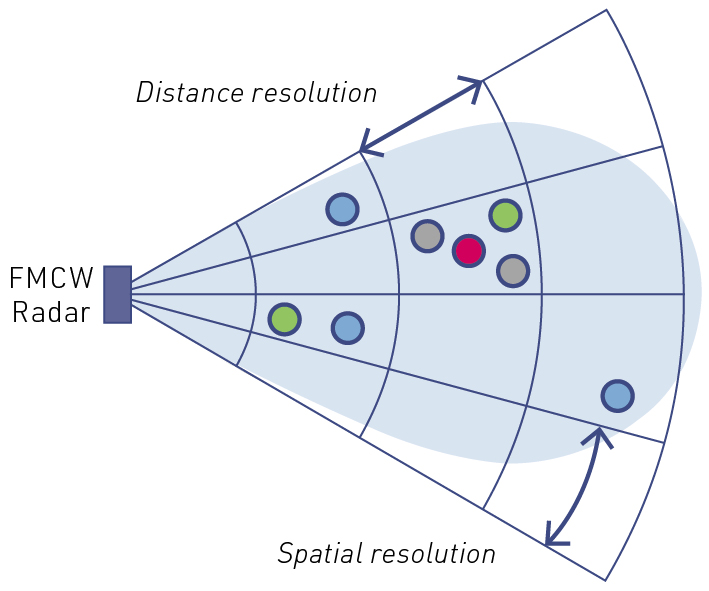
\includegraphics[height=10cm,width=12cm]{Images/chapter2/2-2.jpg}
\caption{تشخیص و تفکیک اهداف مختلف در میدان دید رادار \lr{fmcw}
\cite{rfbeam2024}
}
\end{figure}
\end{center}
\vspace{2cm}

برای دقیق‌تر کردن اندازه‌گیری فاصله در رادارهای \lr{FMCW}، افزایش پهنای باند سیگنال چیپ اهمیت ویژه‌ای دارد. همان‌طور که در مقاله \cite{neemat2019reconfigurable} اشاره شده است، با افزایش پهنای باند \lr{$B$}، دقت تفکیک فاصله بهبود می‌یابد، چرا که تفکیک فاصله \lr{$\Delta R$} به‌طور معکوس با پهنای باند نسبت دارد:
\begin{equation}
\Delta R = \frac{c}{2B}
\label{eq:range_resolution}
\end{equation}
\addequation{رابطه‌ی تفکیک فاصله‌ای برحسب پهنای باند}

این ویژگی، به‌ویژه در کاربردهایی مانند اندازه‌گیری ضربان قلب، که تغییرات فازی کوچکی به‌دلیل حرکت قفسه سینه به وجود می‌آید، بسیار حیاتی است.

\subsubsection{آشکارسازی سرعت} % Corresponds to 2.1.2.2
\label{sec:velocity-detection}

در رادار \lr{FMCW}، سرعت اهداف به کمک اثر داپلر (\lr{Doppler Effect}) و تحلیل فرکانس داپلر استخراج می‌شود.سیگنال‌های بازتابی از اهداف متحرک موجب تغییر در فرکانس آن‌ها می‌شوند که این تغییر به‌عنوان تغییر فرکانس داپلر در سیگنال دریافت‌شده ظاهر می‌شود. فرکانس داپلر با سرعت هدف مرتبط است \cite{kwak2024adjusting} و به‌صورت زیر محاسبه می‌شود:
\begin{equation}
f_d = \frac{2v}{\lambda}
\label{eq:doppler_frequency}
\end{equation}
\addequation{رابطه‌ی فرکانس داپلر برحسب سرعت هدف و طول‌موج}

که در آن:
\begin{itemize}
    \item \lr{$f_d$}: فرکانس داپلر،
    \item \lr{$v$}: سرعت نسبی هدف نسبت به رادار،
    \item \lr{$\lambda$}: طول‌موج سیگنال رادار.
\end{itemize}

یکی از چالش‌ها در سیستم‌های رادار \lr{FMCW}، محدودیت دامنه سرعت قابل تشخیص است. سرعت‌های بسیار پایین یا سرعت‌های بالا ممکن است باعث شود که سیگنال داپلر تغییرات نامشخص یا حتی معکوس داشته باشد، که در نتیجه منجر به از دست رفتن سیگنال یا کاهش دقت در تشخیص سرعت می‌شود.
برای حل این مشکل، مقاله \cite{kwak2024adjusting} به تکنیک‌هایی برای نمونه‌برداری انتخابی (\lr{Selective Sampling}) اشاره کرده است که با تنظیم فواصل نمونه‌برداری، می‌توان دامنه سرعت قابل تشخیص را افزایش داد. به این معنا که می‌توان سیستم رادار را طوری تنظیم کرد که دامنه‌ای گسترده‌تر از سرعت‌ها را با دقت بیشتری اندازه‌گیری کند، بدون اینکه از کیفیت اندازه‌گیری فاصله کاسته شود.


\subsubsection{پیشرفت‌ها در پردازش دامنه داپلر و فاصله} % Corresponds to 2.1.2.3
\label{sec:advanced-range-doppler-processing}

یکی دیگر از چالش‌ها در سیستم‌های رادار \lr{FMCW}، نیاز به پردازش دقیق و بهینه داده‌ها در دامنه داپلر و فاصله است. مقاله \cite{neemat2019reconfigurable}  توضیح می‌دهد که استفاده از پردازش دامنه داپلر قابل پیکربندی می‌تواند به بهبود تفکیک سرعت و فاصله در سیستم‌های راداری \lr{FMCW} کمک کند. این روش با تنظیم پارامترهای سیستم در هر فریم، به رادار اجازه می‌دهد که دامنه‌های وسیع‌تری از سرعت و فاصله را پردازش کند و در عین حال از تداخل‌های نامطلوب جلوگیری کند.
پردازش دامنه داپلر به سیستم‌های راداری اجازه می‌دهد تا علاوه بر اندازه‌گیری فاصله، سرعت حرکت اهداف مانند حرکت قفسه سینه در هنگام ضربان قلب را به‌طور دقیق شبیه‌سازی و اندازه‌گیری کنند. این قابلیت برای کاربردهای پزشکی مانند پایش ضربان قلب در شرایط مختلف حرکت یا تغییر موقعیت بدن، به‌ویژه در مواقعی که حرکت‌های بدن موجب اختلال در سیگنال می‌شود، بسیار مفید است.


%=================================================================================================


